\chapter{Конструкторский раздел}

В данном разделе будут спроектированы схемы алгоритмов, произведена оценка трудоемкости алгоритмов, описаны используемые типы данных, а также произведена оценка памяти и описана структура ПО.

\section{Схемы алгоритмов}

На рисунках 2.1 - 2.4 представлены схемы рассматриваемых алгоритмов.

\newpage 
\begin{figure}[H]
	\begin{center}
		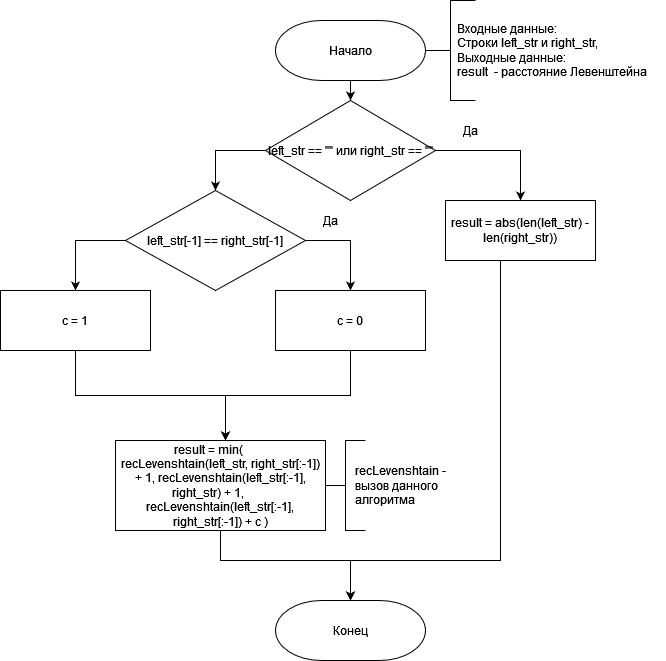
\includegraphics[scale=0.6]{assets/recLevenshtain.png}
	\end{center}
	\caption{Схема рекурсивного алгоритма поиска расстояния Левенштейна}
\end{figure}

\newpage 
\begin{figure}[H]
	\begin{center}
		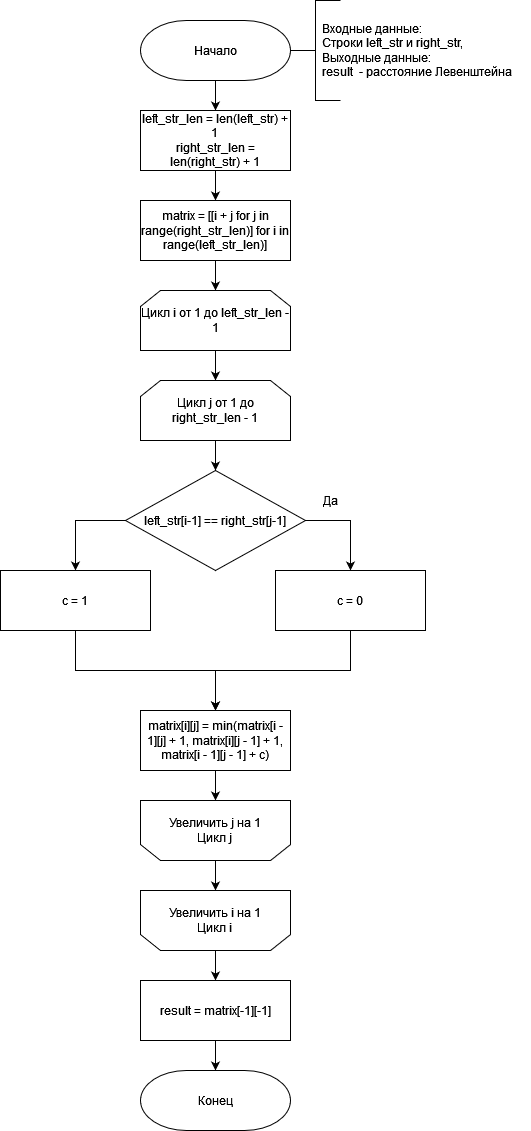
\includegraphics[scale=0.6]{assets/cacheLevenshtain.png}
	\end{center}
	\caption{Схема кеширующего алгоритма поиска расстояния Левенштейна}
\end{figure}

\newpage 
\begin{figure}[H]
	\begin{center}
		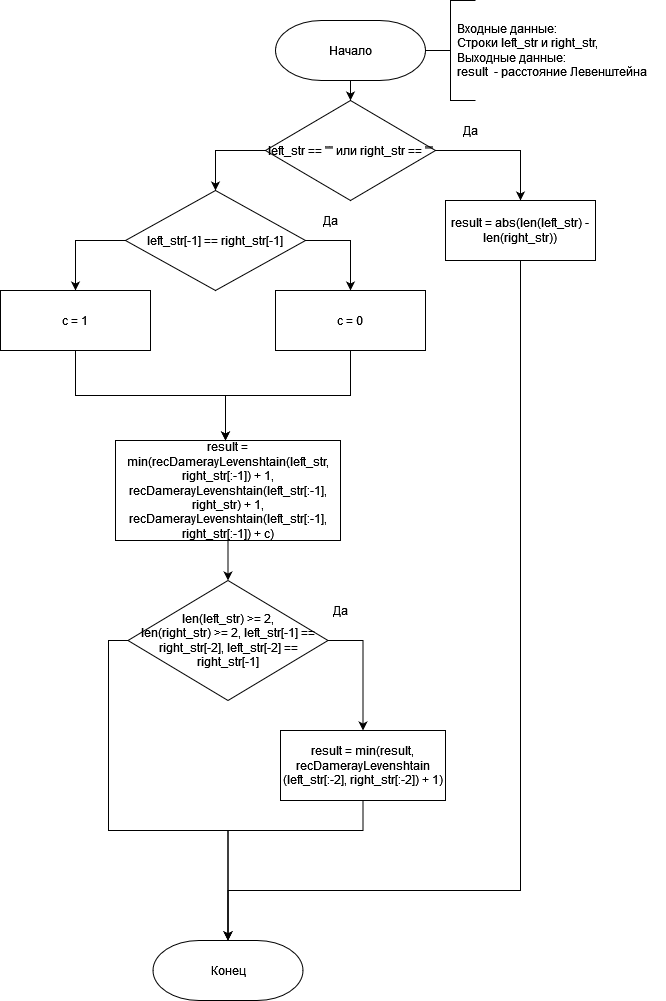
\includegraphics[scale=0.6]{assets/recDamerayLevenshtain.png}
	\end{center}
	\caption{Схема рекурсивного алгоритма поиска расстояния Дамерау-Левенштейна}
\end{figure}

\newpage 
\begin{figure}[H]
	\begin{center}
		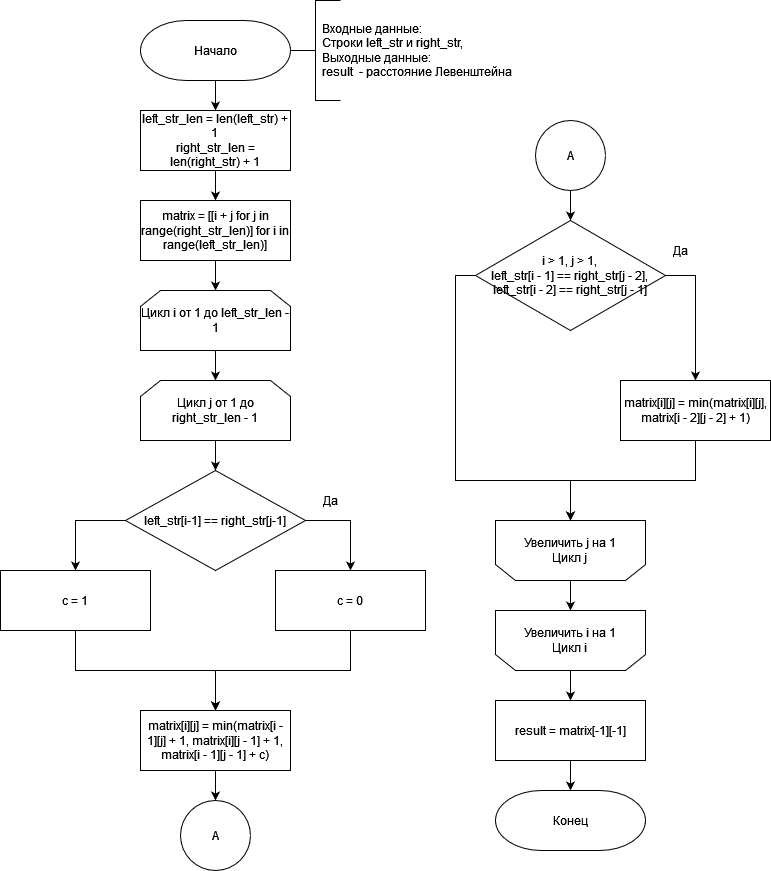
\includegraphics[scale=0.6]{assets/cacheDamerayLevenshtain.png}
	\end{center}
	\caption{Схема кеширующего алгоритма поиска расстояния Дамерау-Левенштейна}
\end{figure}

\newpage
\section{Описание используемых типов данных}

При реализации алгоритмов будут использованы следующие структуры данных:
\begin{itemize}
	\item строка типа str заданного размера;
	\item длина строки - целое число типа int;
	\item кэш в форме матрицы - матрица типа int.
\end{itemize}

\section{Структура ПО}

ПО будет состоять из следующих модулей:
\begin{itemize}
	\item main.py - модуль, вызывающий загрузку меню (является модулем запуска);
	\item menu.py - модуль, содержащий меню пользователя;
	\item myio.py - модуль, содержащий функции формирования строк;
	\item edit\_dist.py - модуль, содержащий функции подсчета редакционного расстояния;
	\item plot.py - модуль, содержащий функции для построения графиков сложности подсчета редакционного расстояния.
\end{itemize}

\section{Вывод}

На основе полученных в аналитическом разделе знаний об алгоритмах были спроектированы схемы алгоритмов, выбраны используемые типы данных, а также описана структура ПО.